\documentclass[border=6pt]{standalone}
\usepackage{tikz}
\usepackage[edges]{forest}
\usetikzlibrary{arrows.meta,positioning,calc,decorations.pathreplacing,shapes.geometric}
\begin{document}
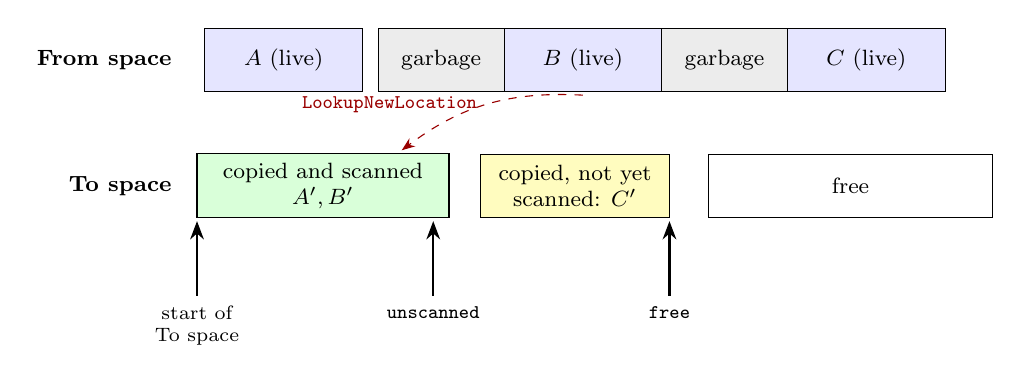
\begin{tikzpicture}[>=Stealth,font=\small,
 cell/.style={draw,minimum height=0.8cm,align=center,font=\footnotesize}]
\node[font=\footnotesize\bfseries,anchor=east] at (-0.3,1.6) {From space};
\node[cell,minimum width=2.0cm,fill=blue!10] at (1.0,1.6) {$A$ (live)};
\node[cell,minimum width=1.6cm,fill=gray!15] at (3.0,1.6) {garbage};
\node[cell,minimum width=2.0cm,fill=blue!10] at (4.8,1.6) {$B$ (live)};
\node[cell,minimum width=1.6cm,fill=gray!15] at (6.6,1.6) {garbage};
\node[cell,minimum width=2.0cm,fill=blue!10] at (8.4,1.6) {$C$ (live)};
\node[font=\footnotesize\bfseries,anchor=east] at (-0.3,0) {To space};
\node[cell,minimum width=3.2cm,fill=green!15] (sc) at (1.5,0) {copied and scanned\\$A', B'$};
\node[cell,minimum width=2.4cm,fill=yellow!25] (us) at (4.7,0) {copied, not yet\\scanned: $C'$};
\node[cell,minimum width=3.6cm] (fr) at (8.2,0) {free};
\draw[->,thick] (-0.1,-1.4) node[below,font=\scriptsize,align=center]{start of\\To space} -- (-0.1,-0.45);
\draw[->,thick] (2.9,-1.4) node[below,font=\scriptsize]{\texttt{unscanned}} -- (2.9,-0.45);
\draw[->,thick] (5.9,-1.4) node[below,font=\scriptsize]{\texttt{free}} -- (5.9,-0.45);
\draw[->,dashed,red!60!black] (4.8,1.15) to[bend right=20] node[left,font=\scriptsize]{\texttt{LookupNewLocation}} (2.5,0.45);
\end{tikzpicture}
\end{document}
